\chapter{Protein Structure}
\section{Protein Structure - Lecture 4}

\subsection*{The Classical Structure-Function Paradigm}
\begin{figure}[h!]
    \centering
    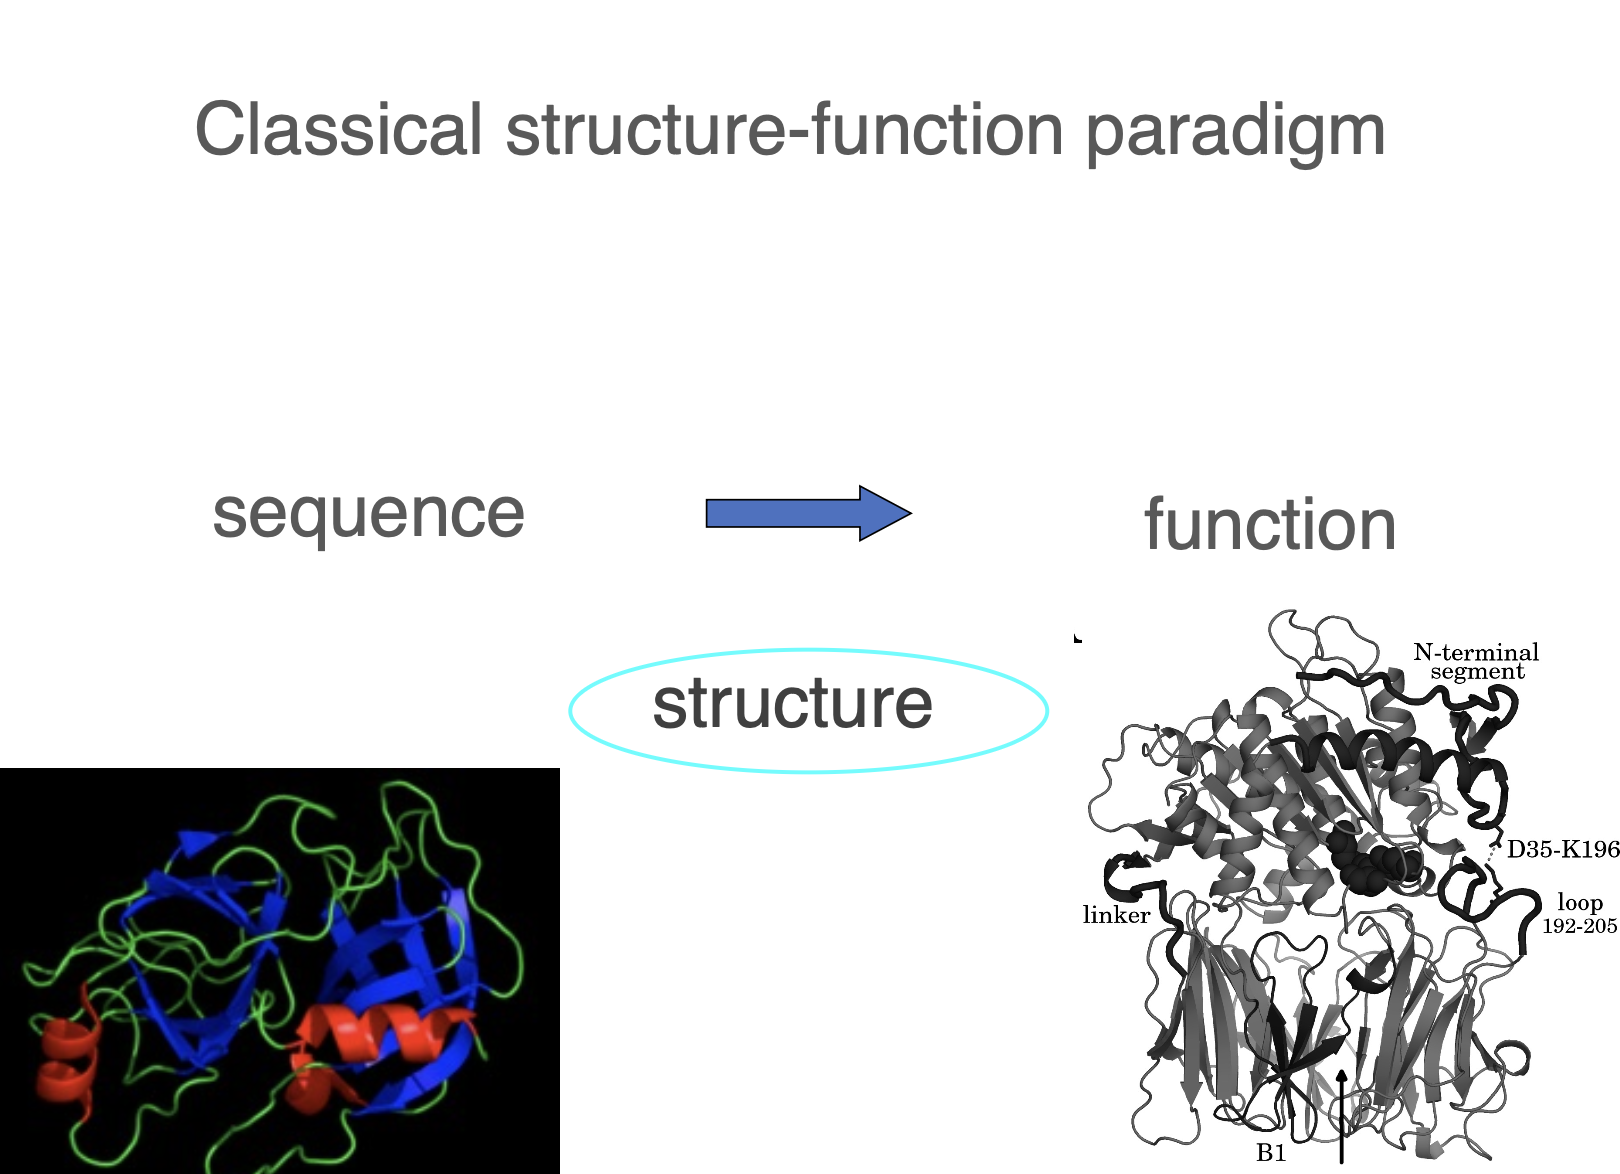
\includegraphics[width =0.8\linewidth]{slides/protein_structure/classical_structure_function_paradigm.png}
    \caption*{}
    \label{fig:placeholder}
\end{figure}

\noindent People work with this. It's called a classical structure-function paradigm, and they believe that the protein sequence encodes the function through a well-defined structure of a protein. What you need to see as a physicist is that this is a \textbf{deterministic relationship without any uncertainties}. This is what biologists believe in, this is what chemists believe in, and this had been a very strong constraint on the whole field of biology, and this is what gives you opportunity to work in the coming decades and a good salary or gain good research reputation, whatsoever. \textbf{The fact that this is not true.} This is your future. What you need to understand, again as a physicist, that this is a deterministic relationship making no notions whatsoever things that, for example, these entities, sequence, function or structure, can be \textbf{ensembles}. 


\subsection*{Learn how to read sequences}
\begin{figure}[h!]
    \centering
    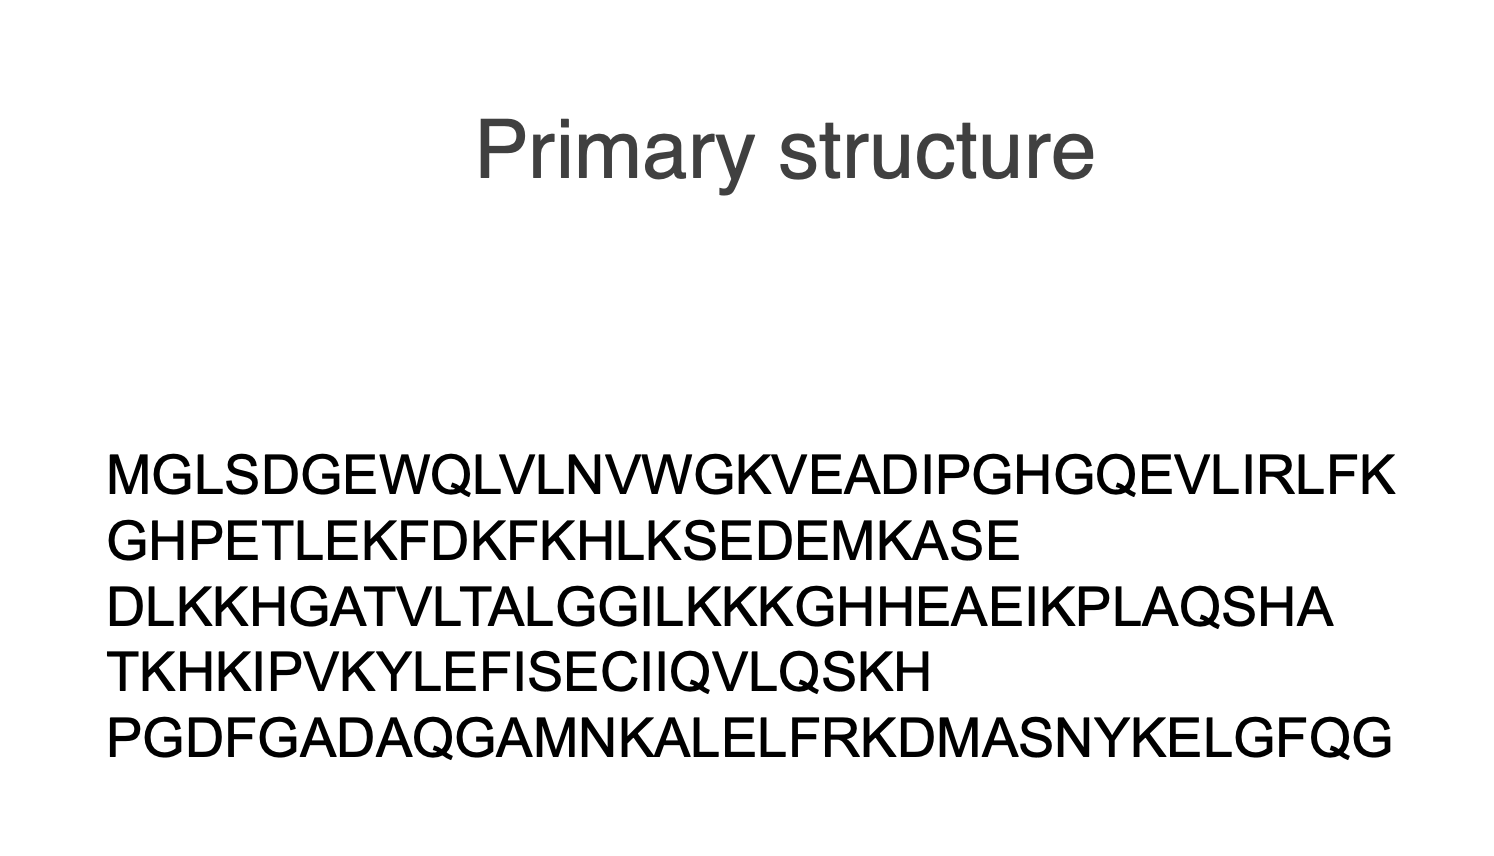
\includegraphics[width =0.8\linewidth]{slides/protein_structure/PRIMARY_STRUCTURE.png}
    \caption*{}
    \label{fig:placeholder}
\end{figure}
Let's start with the primary structure. \textbf{The very first thing I suggest you to do is to learn what the letters mean.}  Because you need to read it. Try to read it with your, I mean, with your intuition, nd try to note something. Believe me or not, I'm working with proteins kind of every day, and I am reading these. And sometimes from my own reading understand something, because why? Because the brain does some kind of well, intelligence. So, let me help you, let me teach you to read. 
\smallskip \newline \noindent
If you look the whole text, do you find more or less the 20 letters? I mean, just as a first sight. Yeah, I mean, there is quite a bit of variations, maybe you don't need to there is quite a bit of variation in the letters. This we can say. Then, you know, if I start reading it, there is one follows another, so it's not the same letter. So, it's there are different letters. And then you keep reading, and then you let's say arrive at this line, you say KK and GG and KKK, even three the same. So, there are some things which are kind of repetitive. 

\subsection*{The Aminoacids}
\begin{figure}[h!]
    \centering
    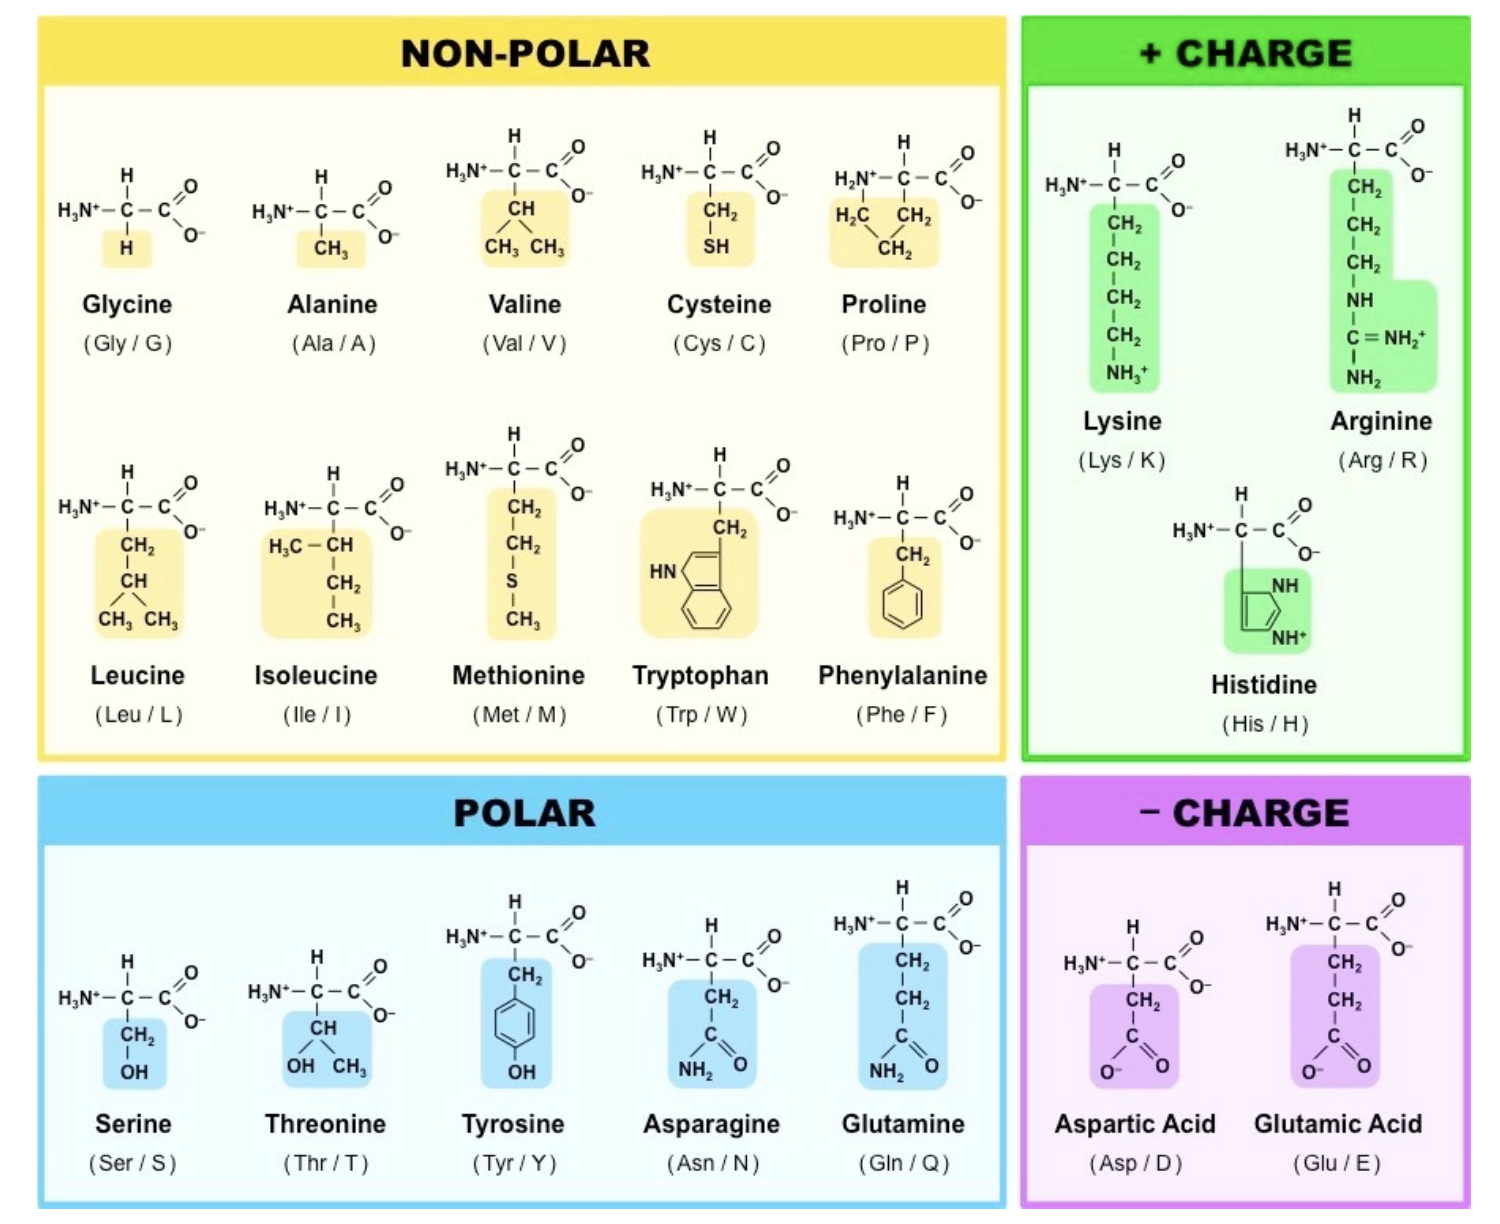
\includegraphics[width =\linewidth]{slides/protein_structure/aminoacid_table.png}
    \caption*{}
    \label{fig:placeholder}
\end{figure}
So, we have 20. All the 20 have different properties. Now, this  picture  I suggest you to print out and put above your tables when if you really start doing some biological calculations. 
\paragraph{Polar and Non-Polar}
You see here words non-polar and polar. This means polar ones like water, non-polar ones don't like water, they prefer oil. I will only speak about very simple things and keep yourself simple even to do the best machine learning in the world. Okay? You don't have to be complicated, you just have to be clever.

You see that you have lots of non-polar I mean, if you just again, briefly look at the numbers, you the the largest group is the non-polar. \textbf{Why?}

 So, at the end of the day, we construct proteins that are several hundred residues, let's say. Most of them are compact. So, we have to get them compact. We construct them in a water-like environment. So, we have to make them compact. Now, if we put all the polar and later on charge, I they like water so they don't want to be compact simply. 

\paragraph{Protein Charge depends on pH}
We say charged, but it depends on which solution they are or which protein they are. I mean if you put the pH very high, then, you know, everything will be deprotonated. If you put the pH very low, then everything will be protonated. So, you know, it depends. So we can say it's charged, but when you compute machine learning, you have to put one number at that pH or at that protein or at the cytosol or somewhere. So this is not an absolute quantity, this is what I'm trying to tell you. 

\subsection*{Useful Properties of some Aminoacids}

I'm trying to call your attention to some properties that you may pick up when you do the machine learning. All amino acids are very special,we have to pick up their speciality, and understand if it's relevant to the problem that we are studying.

Coure
\begin{figure}[h!]
    \centering
    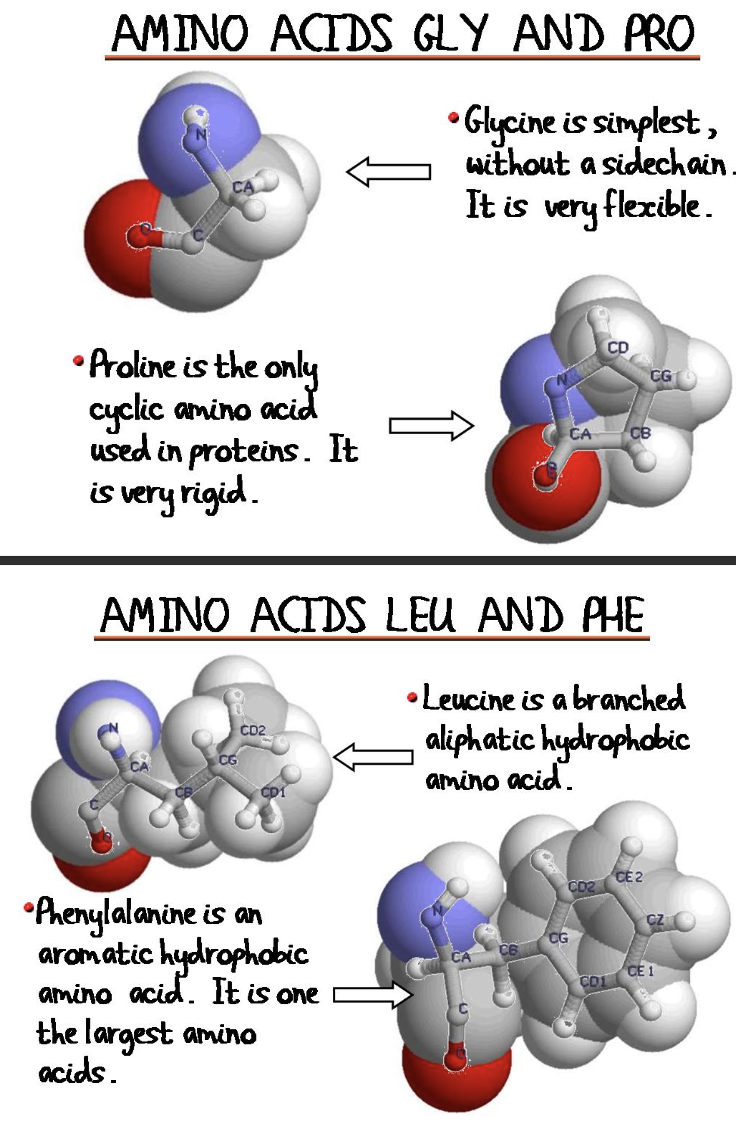
\includegraphics[width =0.48\linewidth]{slides/protein_structure/gly_pro.png}
    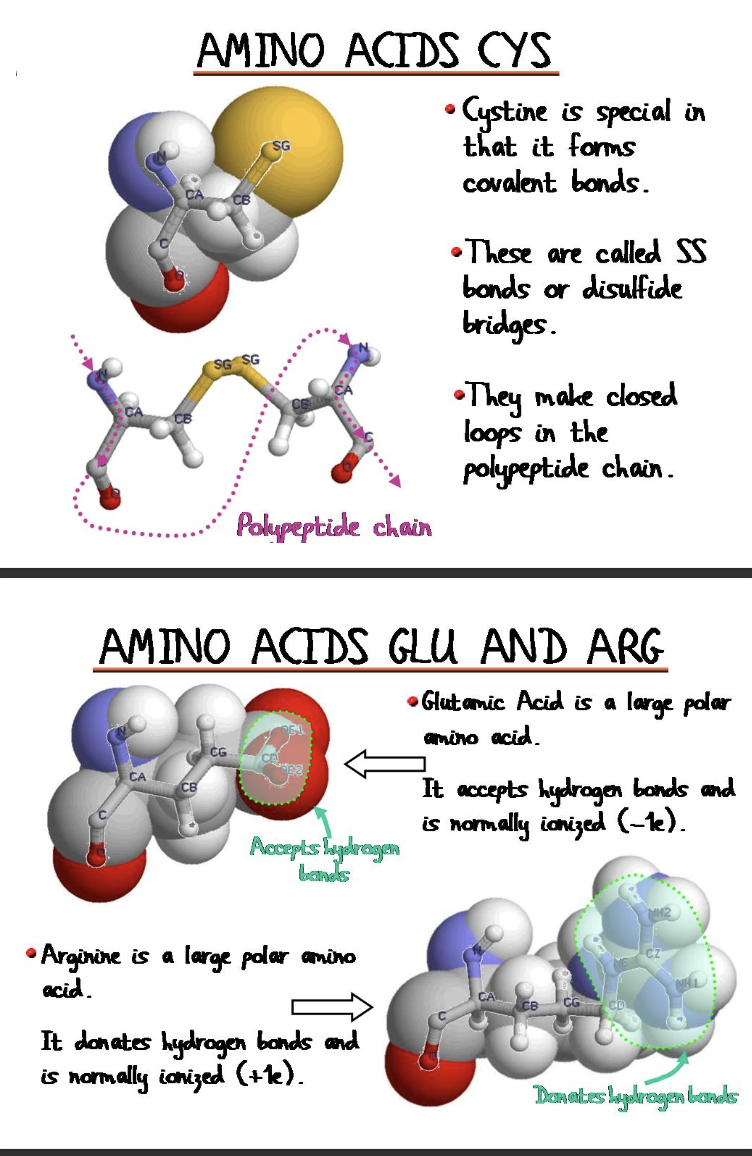
\includegraphics[width =0.48\linewidth]{slides/protein_structure/cys_arg.png}    
    \caption*{}
    \label{fig:placeholder}
\end{figure}


\paragraph{Glicine}
Glicine is the simplest amino-acid. Its side chain only consists of one hidrogen atom. This has two important consequences:
\begin{itemize}
    \item it is very mobile and flexible,
    \item it is not chiral
\end{itemize}
Flexibility implies that glycine is very involved in some processes, for example if you learn about transcription, transcription is a super dynamical process. The enzymes that are doing it must have some tails, some parts that are full of glycines because it must be very flexible. 


\paragraph{Proline}
Then we have proline here. Now, proline is also very special. There is a covalent bond between the end of the side chain and the main chain. It is the only cyclic aminoacid that is used in proteins. Chemically actually it's called an imino-acid, it's not even an amino acid, but this question we ask only from the medical students if you want them to fail the exam.
But what is important for you is that this is a big constraint: somehow it limits the conformations and basically it will restrict \textbf{proline to two main states. cis and trans} - more on that later. So things that want to change their function in a kind of binary manner would use proline because once in this state, once in the other state, only because of that constraint. 

\paragraph{Cystine - Dsulfide bridges}
 I take another amino acid—I won't go all through the twenty, I'm just giving you flavors. I take another which is called cysteine and cy—normally most of the side chains, if you look carefully, have a carbon, have oxygen, and nitrogen, these three. And hydrogens, of course. \textbf{This one also has a sulfur}. Big—first of all, you can see it's big, bigger than the others. Otherwise, there is another amino acid which is about the same size just there is oxygen here. Why it's interesting to have the sulfur? But the sulfur is a very sensitive atom in a sense that \textbf{it can be SH if it's reduced, and it can be SS - sulfur bound covalently to a sulfur - if the conditions are oxidizing}. Having said that, since this is, you know, on one part of the main chain, maybe, you know, the other is on a completely different part of the main chain, through this kind of bonds, which are covalent bonds again, formed only if the conditions are proper, you can put a strain. When you form a covalent bond, you make a strain. You put a strain on the whole protein, you stabilize it, and many cases you have the situation when—I mean you—you have a protein, you know, something, and you cut it, actually it's happening in your stomach for example. You cut, but it doesn't fall apart because there is this kind of bond. Before this kind of bond is formed, and then you can cut the chain. 

\paragraph{Phenylanine (F)}
 You can see that there is a ring here. You can see that there are six members and the particular feature of those six is that they are \textbf{planar}. There are two energetically favoured conformations of mutliple phenylanines: You can make of course a sandwich (\textbf{think about protein condensates!}), but the other is a T-conformation, this is energetically favored. This means that here you can very easily generate multiple states in a very easy manner. Because the benzene ring has a cloud of delocalized electrons above and below its plane (the $\pi$ system), Phenylalanine residues like to "stick" to each other or other aromatic residues (Tyrosine, Tryptophan):
\begin{itemize}
    \item The Sandwich (Parallel Stacking): Two rings sit flat on top of each other. While common in textbooks, this can actually be less stable due to electron repulsion between the clouds.
    \item The T-shape (Edge to Face):  The slightly positive edge (hydrogens) of one ring points into the slightly negative face ($\pi$ cloud) of the other.
\end{itemize}
\paragraph{Leucine}
You see the leucine, we say it is branched, because here there is a branch. Why it's important? \textbf{Well, when it's branched, I mean it can occupy more space, and there can be more water released to the bulk, this kind of things.}
\paragraph{Glutamic Acid}
There is another residue which is negatively charged, which is one carbon less, so only this one and the carboxylate group comes immediately, that is called aspartate. You can ask immediately, why nature created two which are more or less the same? Not the same, because one can be protonated at a pH of four point three and the other at three point nine. This is aspartate and this is glutamate. They—it absolutely sets them for different enzymatic reactions. Nature played a lot in which cases uses glutamate, which cases uses aspartate. They many times participate in we call proton shuttling: they get a proton, get neutral, give up a proton, and so on. So that's an interesting property. 
\paragraph{Arginine}
 You see that there are three nitrogens here, center in the center there is a carbon, and the whole thing you may imagine as here it's—it's planar. Again, it's full of delocalized electrons. 
For a long time, many decades, we didn't care that much about arginine. And suddenly, like ten years ago, more or less ten years ago, we got interested in arginine. Why? Because people discovered—I mean it's—it’s stupid—but people discovered that arginine has this delocalized electrons, and similarly what I explained about phenylalanine, it can make the sandwich, it can make the T-conformation. And what they realized first it was from machine learning, that this arginine is very important to form the protein condensates, this droplets in the cell. But they didn't understand why. So they had to go back to elementary chemistry. So it was first came out from machine learning really, published big journals, you know: the arginine is important. 
\subsection*{Amino-acid Classification}
\begin{figure}[h!]
    \centering
    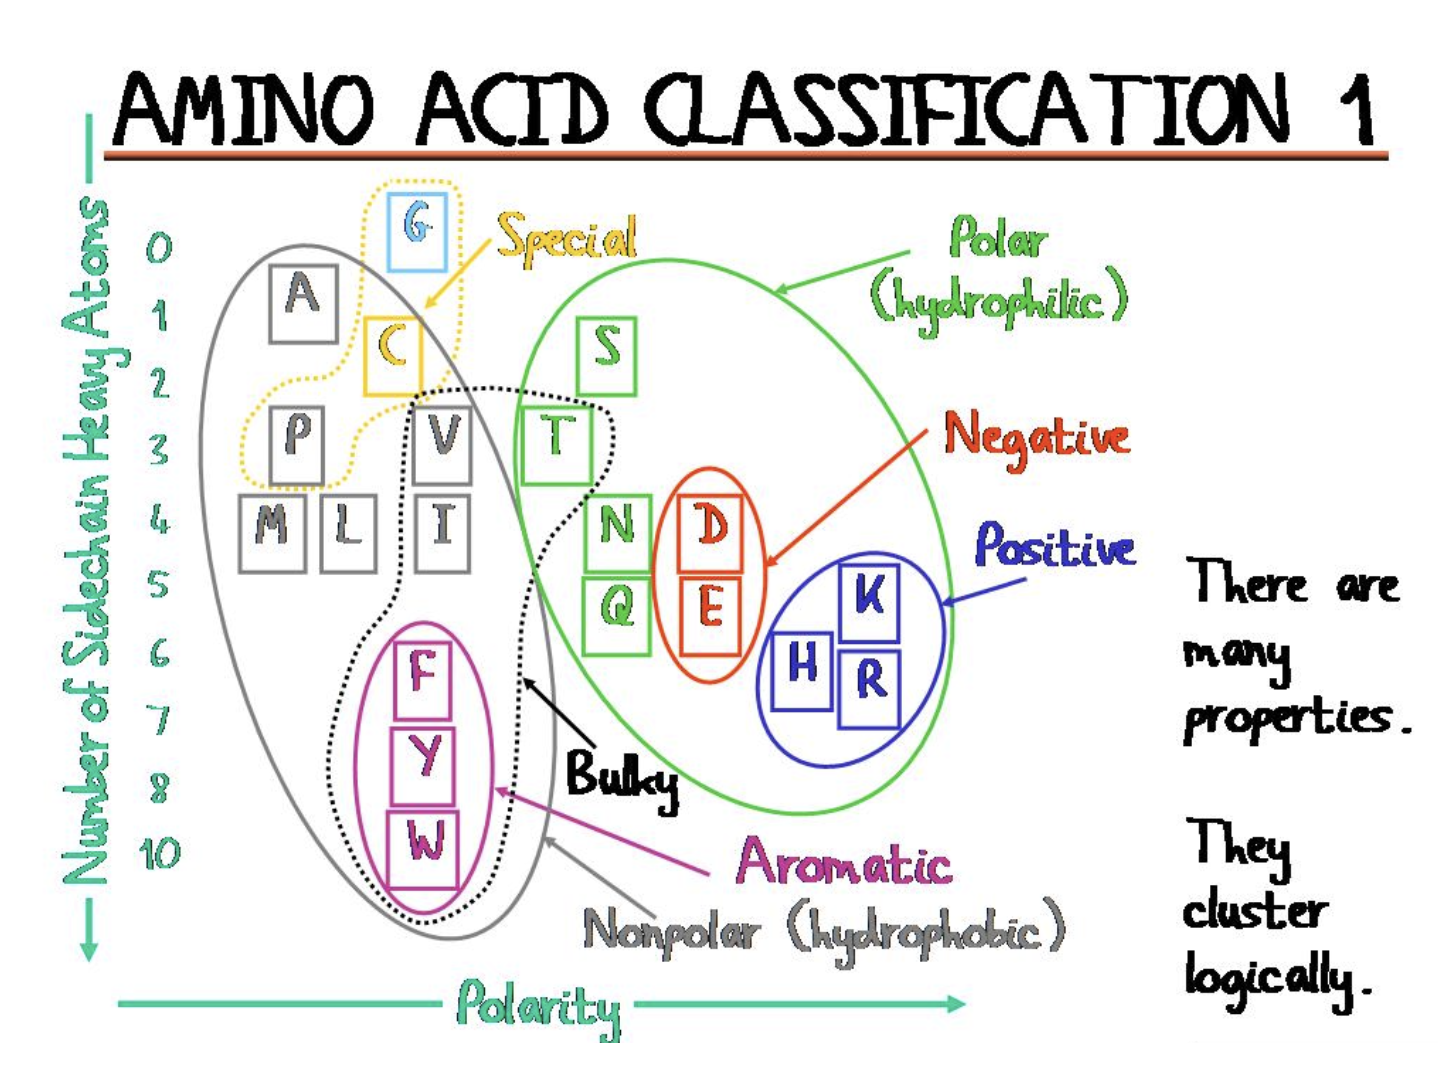
\includegraphics[width =0.8\linewidth]{slides/protein_structure/aminoacid_classification.png}
    \caption*{}
    \label{fig:placeholder}
\end{figure}

\begin{itemize}
    \item \textbf{Low polarity, many heavy atoms} So anyway, uh, so what can you expect from this group, for example, which are have a low polarity and have many heavy atoms? What—what do you expect based on the knowledge you have already, let’s say? They would attract many non-polar molecules to themselves. So they would—they would have the compactness, right? You would expect that they would be inside, maybe, of this compact issue, right? 
    
    \item  And then you can come to here and what you expect, these are the positively charged ones, this is arginine and this is also a ring-containing compound. What do you expect? You expect either that they stay outside because they like water, or you expect that they would create a very specific environment for some reactions and so on, same as for these one. 
    
    \item \textbf{Serine (S) and Threonine (T) are switches} And more you go towards kind of medium polarities, you would expect kind of ambiguity, so, you know, behave like this, behave like that, behave like this, behave like that. This kind of things nature like, to change something. So these ones, These are small residues, serine and threonine, they
    have a hydroxyl ($OH^{-}$) group. This group is relatively small and neutral, but it is chemically nucleophilic, meaning it’s ready to react. The hidrogen atom in the hydroxyl group can be replaced by a phosphate group ($PO_4^{3 -}$). You go from a small, uncharged, slightly polar residue to a huge, bulky, doubly negative group. This massive change in charge and size usually causes the protein to "snap" into a different shape, \textbf{turning an enzyme "ON" or "OFF."} This is the basis of nearly all cellular signaling.
     Nature likes regulation, it's very important for complex organisms. It's all about regulation, not about the number of genes, not about the length, not about nothing else, it's about regulation So these ones, that get this post translational modification, they change and then they make something. For example, they pass the signal, they get a phosphate and then the phosphate is taken off.
    
    \item \textbf{Asparagine (N) and Glutamine (Q)}
    These are the neutral versions of Aspartic Acid and Glutamic Acid: they have an amine group ($NH_2$) where the others have a carboxyl group.
These two are very dangerous. They- they make amyloid aggregates that I explained later, it's more complicated. Basically, if they are over-represented in a protein sequence, they can zip together into indestructible fibers called \textbf{Amyloids}. This is the structural basis for diseases like Alzheimer’s or Huntington’s.

\subsection*{Sequence Complexity predicts Disorder Degree}

\paragraph{An ordered one: Myoglobin}

\begin{figure}[h!]
    \centering
    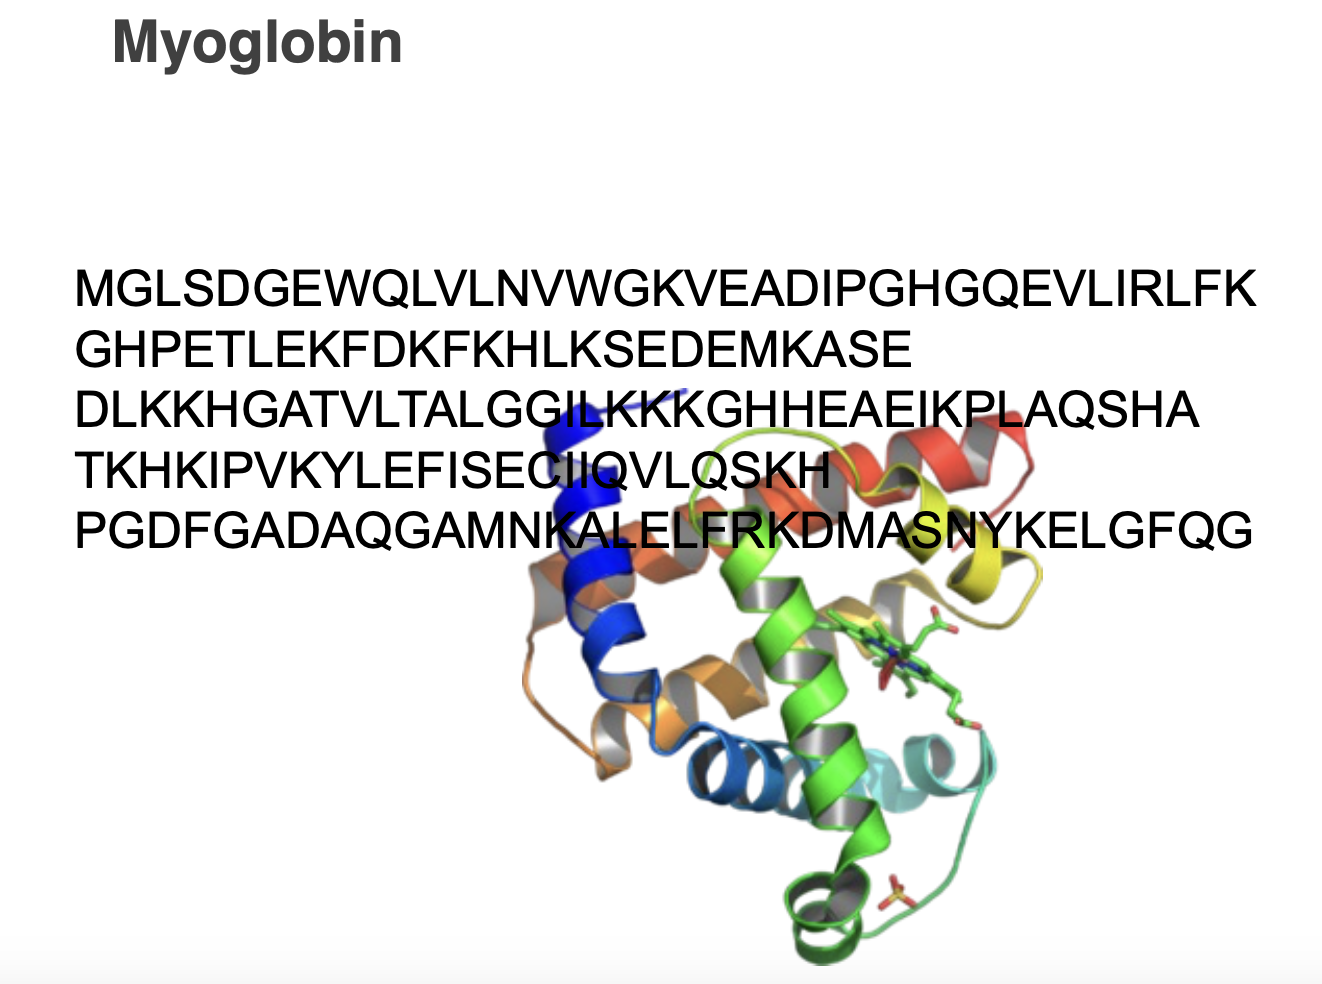
\includegraphics[width =0.8\linewidth]{slides/protein_structure/myoglobin.png}
    \caption*{}
    \label{fig:placeholder}
\end{figure}

There are quite many of these twenty, almost probably all of them are represented here. There are not many repetitions. \textbf{So we can make a conclusion- I mean, it's an early conclusion but- but try to see the- the correlations between things. That if I have many, I have quite nice structure}, so it's- it's quite well defined, even this perpendicularities (between helices) is important, it's- it's quite well defined. 

\paragraph*{A messy one: the Mastermind}

\begin{figure}[h!]
    \centering
    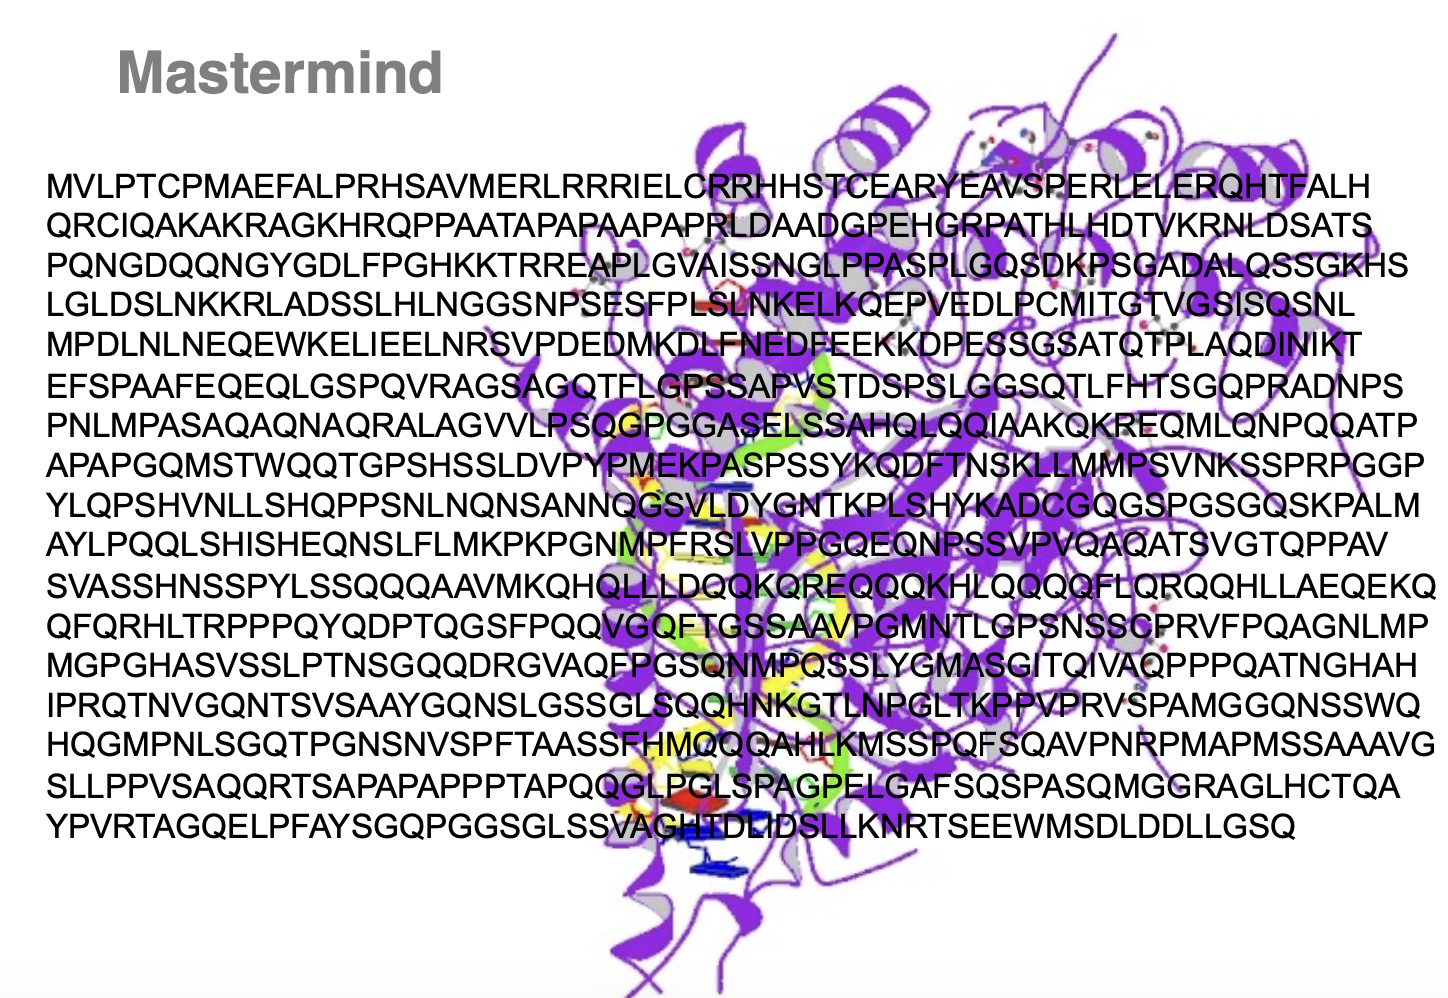
\includegraphics[width =0.8\linewidth]{slides/protein_structure/mastermind.png}
    \caption*{}
    \label{fig:placeholder}
\end{figure}

Now I show you another protein. It's- it's messy basically. Try to read again and tell me something about your reading experience.

Student: There are more repetition in the letters. Repetitions involves different letters

Speaker: Different but not - not any kind, right? That- there are some that are distinguished in this repetition, no? This we note. Like for example, \textbf{G,Q}, \textbf{S,S,S} . And when S is repeated, then many times there is a G there, so there is an associated G. Or if you look, another times there's an associated R.


\paragraph*{A messy one that creates condensates}

One of the key proteins of the ALS disease, the Amyotrophic Lateral Sclerosis. Um, this means you have a single mutation, one amino acid changed, and it starts to grow like a hedgehog. If you don't have a single amino acid mutation, it stays normal like this. 

Speaker: But read the letters. Read the letters. What do you notice?

Student: There are a huge repetitions.

Speaker: What kind of? G,G,G and what else? Q, S... if you look very carefully in the region which I highlighted, if you count how many types of residues are present or dominant, it's different than Myoglobin. I don't know, there are maybe five residues here out of the twenty. So not all the twenty are represented. This is very important. 



\paragraph{High-complexity and Low-Complexity Proteins have very different roles}

\begin{equation}
    H(\text{sequence}) = - \sum_{\small \text{Amino- Acids (AA)}} f_i(AA) \cdot \log_2{f_i(AA)} \quad \textit{Shannon Entropy of a sequence}
\end{equation}

\begin{itemize}
    \item high shannon entropy = high variety of aminoacids. These are called high complexity sequences.
    \item low shannon entropy = low variety of amino-acids. These are called low complexity sequences.    
\end{itemize}

So, does it matter? Of course it does matter, otherwise I wouldn't speak about it. 
\begin{itemize}
    \item  \textbf{High complexity proteins: the "Swiss watches"}
     This is the hallmark of enzymes and folded proteins. To catalyze a reaction, you need a highly specific 3D pocket. You might need a Histidine to grab a proton, a Serine to attack a bond, and a Leucine to hold the substrate in place. These residues must be positioned with sub-angstrom precision. If you change even one amino acid (lowering the complexity/variety), the "machine" breaks.

    \item \textbf{Low complexity proteins: morphogenesis} When H(sequence) is low, the protein is repetitive (e.g., Gln-Gln-Gln or Gly-Ser-Gly-Ser). These are often Intrinsically Disordered Regions (IDRs).
    If you are coordinating 1,000 processes at once (like during embryo development or "morphogenesis"), you cannot have $1,000$ rigid machines clashing into each other.
    Low-complexity sequences act more like liquid or velcro. They allow for multivalent interactions: they can bind to many different partners weakly rather than one partner strongly (\textbf{fuzzy interactions}).
\end{itemize}


\paragraph{A sequence could have both low complexity and high complexity domains}

Speaker: So how do you know that this is going to form a droplet and then ages to this hedgehog and then form aggregate? So you want to distinguish these regions. One that will be structured and the other that will not be so structured, or structured only in a case of a pathology. But for example, if you were computing sequence complexities, you should find a great difference in between these two.

\end{itemize}



\section{The Conformational Landscape (Lecture 5)}

\begin{figure}[h!]
    \centering
    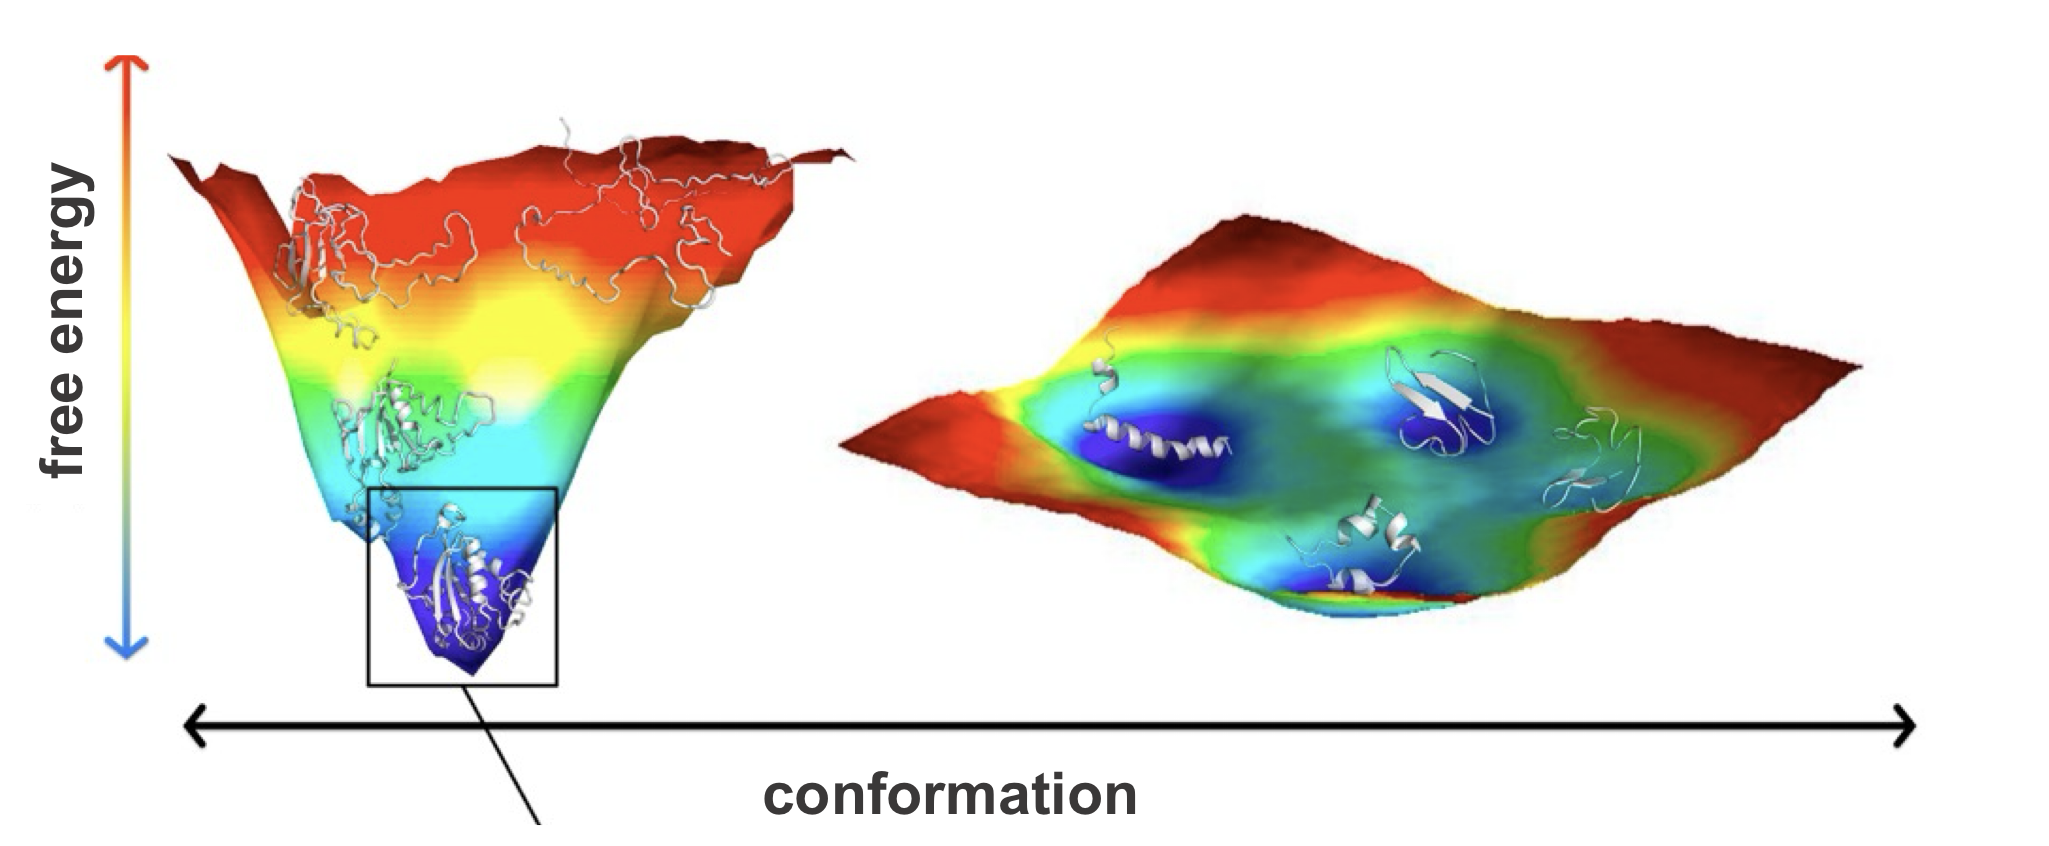
\includegraphics[width =0.8\linewidth]{slides/conformational_ensemble/continuum.png}
    \caption*{}
    \label{fig:placeholder}
\end{figure}

\noindent The folding process is driven by thermodynamics laws: the system (the protein) will spontaneously evolve towards a configuration that corresponds to a (local) minimum of the free energy. In this context, the free energy that we need to consider is Gibbs free energy 
$$
G(T, P, N, \text{other parameters}) = U(S*, V*, N, \text{other parameters}) + PV - TS = H- TS
$$
Spontaneous transformations satisfy $\Delta G = \Delta H - T\cdot \Delta S < 0$. In general, the Gibbs free energy defines a very complex hypersurface,  which we call a \textit{conformational space}. So, this complexity, let's say, faces a protein with a challenge that you will feel immediately once you push the first "start" button into your simulations, because you will see that it doesn't want to converge, there are many bottlenecks at some points that you just cannot pass.

\noindent Sometimes it is a real challenge, for a protein, to reach an \textbf{adequate state}, meaning a state where it can function properly. Notice that I used the word "adequate" - not \textbf{"native"} - as you find in the literature, to avoid two common misconceptions:

\begin{enumerate}
    \item the state where the protein can function is unique (FALSE)
    \item this state corresponds to the global minimum of the free energy (FALSE)
\end{enumerate}
These false beliefs have been around in the field for decades, and it is better for you to learn the reality from the very beginning. People made some early on experiments trying to heat up proteins a little bit and then let them cool. And what they experienced, that they always get back to the same state, and this is why they thought, "Oh, there is just one of these states and the protein must find it." And for example, just to tell you why you must be cautious with this notion, that for example in your cells, in your body, the most stable state for proteins is an \textbf{amyloid state}, which is in most cases not functional but pathologic. And it is also irreversible. So, that’s kind of a dead end for a protein. 

\paragraph{The landscape is not a flat golf course (oh, really!?)}
At first, people had this naif idea that the native state was unique and that the energy landscape was kind of flat, with a very sharp dipping point where the native state was. But if things where like that, then doing very simple calculations, you can see that the average time for the folding process to complete would be large than the age of the universe! Instead, proteins fold in the range of \textbf{milliseconds - seconds}. So this must be clearly false. 

\paragraph{The Funnel idea}
So one of the first answers were coming '87 by Ken Dill, who is still alive and active, and he proposed the funnel. \textit{The funnel means that there is a vast space in the beginning and after a short amount of time, it’s not only time but it’s also the number of the contacts, the protein reaches a state from which there is only one way to achieve the final structure.} So there are multiple pathways here in the beginning and then there is a funnel. By the way, all the AlphaFold is compatible with the funnels, but not with the ensembles. Now there is an AlphaFold multimer, but they are still working on it. I'm stressing it, that would have meant that for a while you have many configurations, but after a while everything is kind of determined for a single state. Okay? Please note—I’m showing quasi each lesson on this structure-to-function paradigm, deterministic—please note that this is a, I don't know, like a rephrased form of that that paradigm. It's absolutely deterministic, at least from from this point.
\begin{figure}[h!]
    \centering
    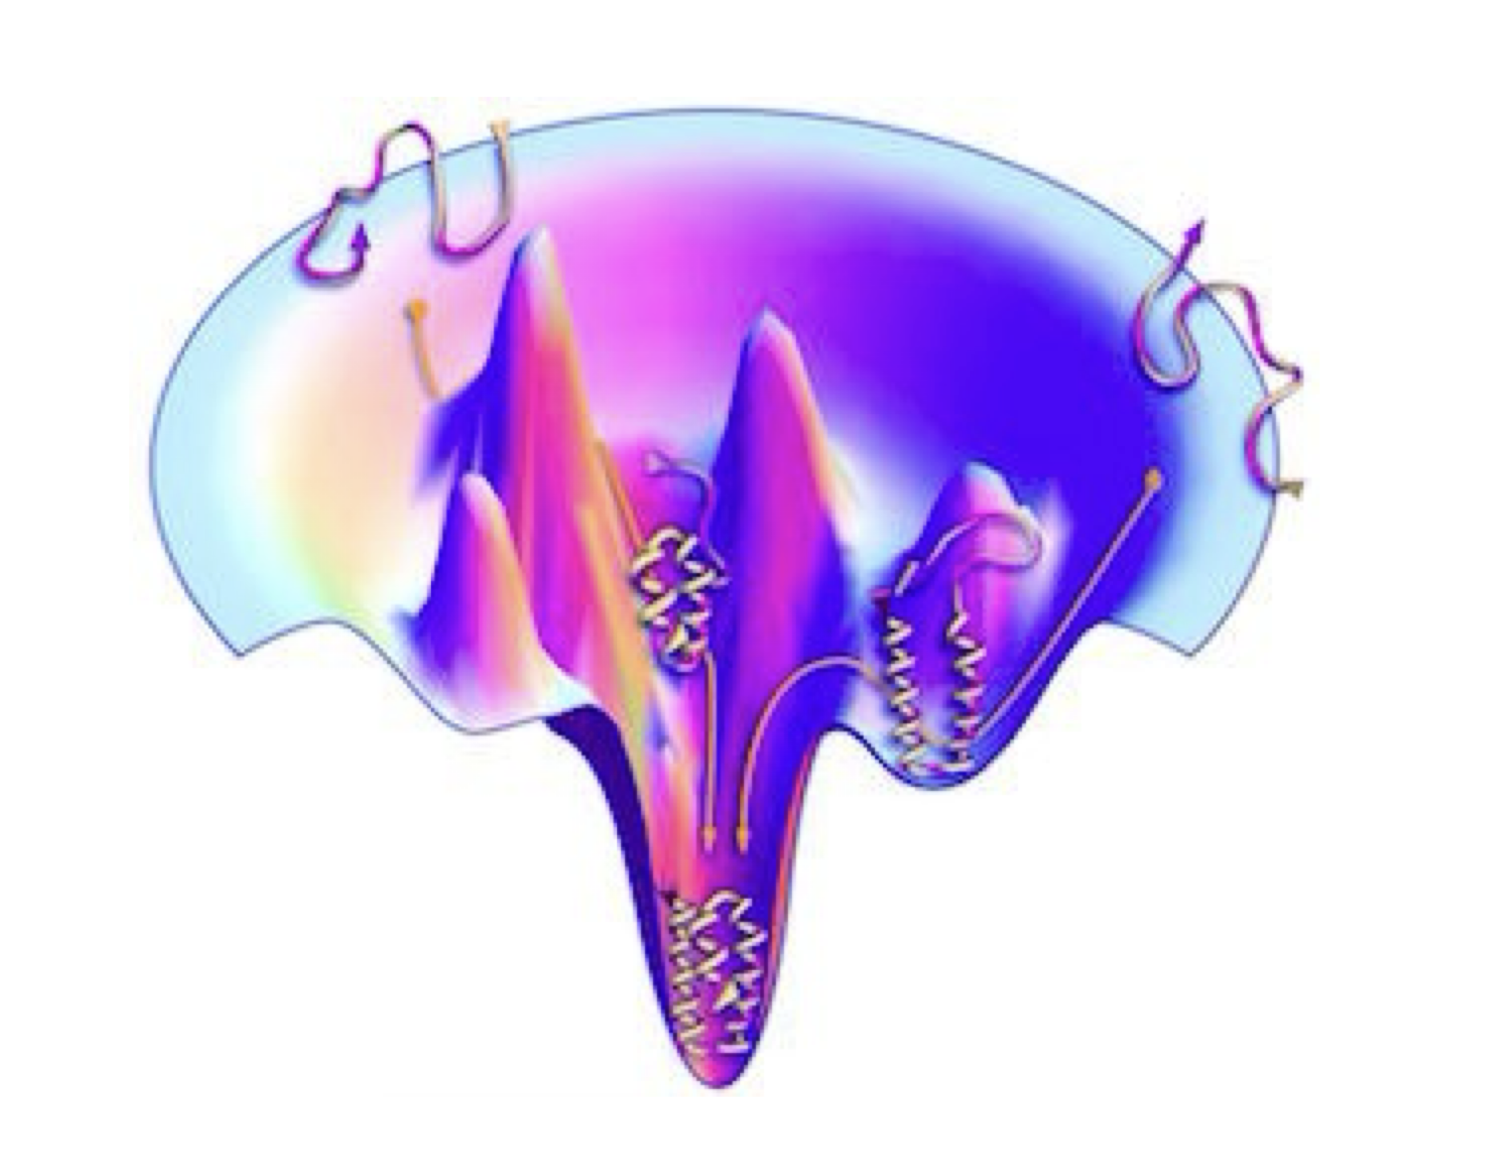
\includegraphics[width=0.3\linewidth]{slides/conformational_ensemble/funnel.png}
    \caption{the funnel model}
    \label{fig:placeholder}
\end{figure}


\paragraph{The reality: frustration}
Twenty-five years ago, people started realizing that some proteins have a pletora of metastable states. They thought it was a special class of proteins, but in fact all the proteins are like this, some more and some less. The landscapes range in a continuum, some are quite sharp, some others are very shallow. And then people started to talk about the spin glass effect in proteins, okay? Obviously this community of physicists. So, what is the spin glass effect? That you you there is frustration, you cannot fulfill all the interactions in a in an optimal way, but you must leave some kind of frustrated, unfulfilled. And these states cause little bit of variation of something that we would call "ideal" or "native". You should not say "that's non-native, so that's not functional" - it is not true. These are marginally stable states here, and you have some conflict in energy. IT doesn't mean that it's non-native; \textbf{it means that it can be native under some different circumstances}. It means that when evolution comes and let's say faces the protein with with something different than it got used to—for example, the temperature gets higher, for example happening now, right? Or the CO2 concentration becomes higher, or thousands of other things, okay?—then the protein can shift towards this.
\begin{figure}[h!]
    \centering
    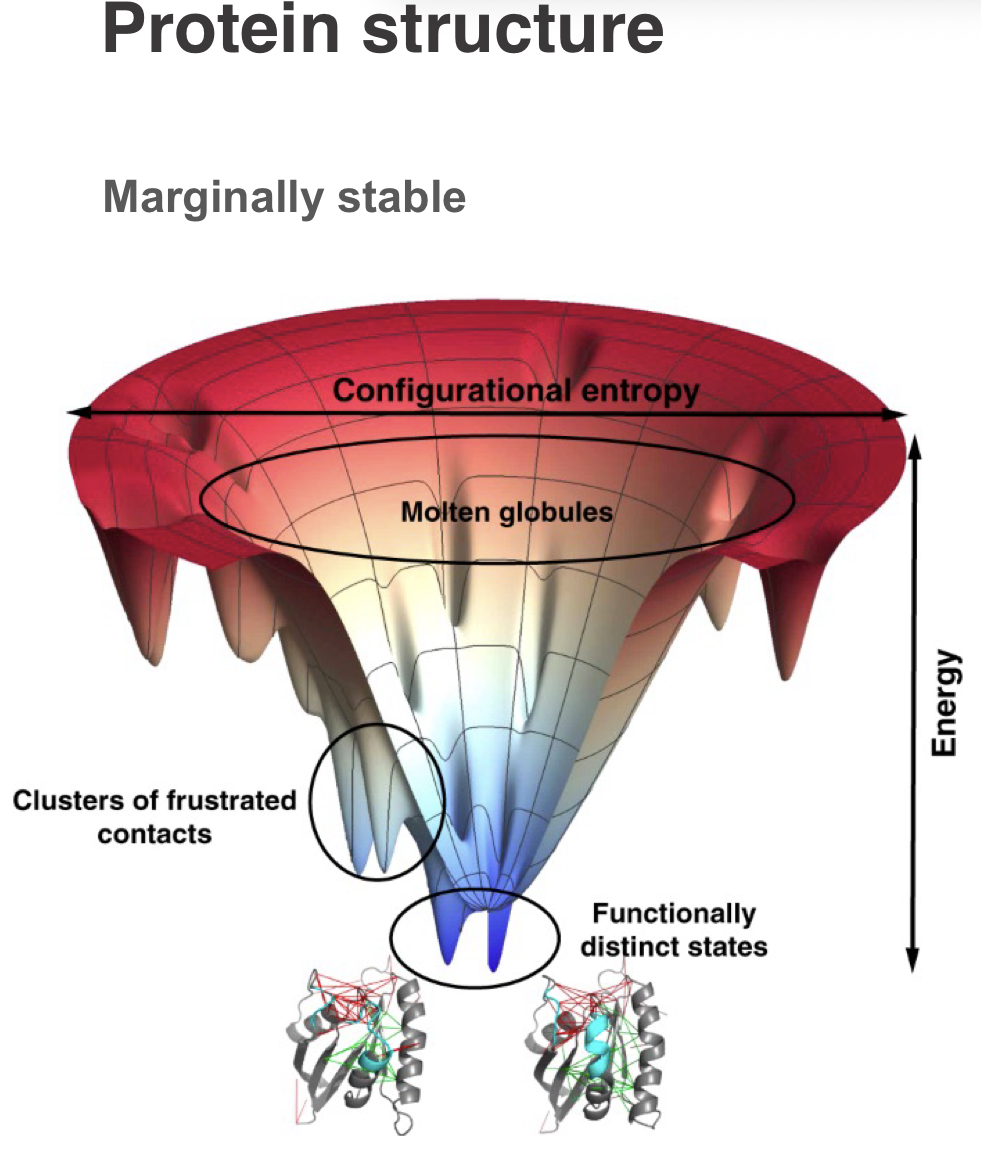
\includegraphics[width=0.3\linewidth]{slides/conformational_ensemble/frustration.png}
    \caption{Frustration}
    \label{fig:placeholder}
\end{figure}
These states are very important. So, the fact that you don't die every day from eating the food that you buy in the supermarket which contain chemicals from pesticides that are absolutely new on earth, like they were discovered 10 years ago whatever. All your proteins were not evolved to deal with this, it's absolutely new, it’s absolutely dangerous for you. But your proteins are very intelligent, they have this state, and because they have this state, this state can degrade this unknown substances, they adapt, and well, you are here, you are listening to me. \textbf{You need to understand that what we call "non-native" is just something that is not the major function, but the protein is evolved to have this kind of secondary activitie}s, moonlight activities, whatever, through the frustration of some of the contacts. Tt’s not random which ones, okay? It’s very important. It would be fantastic to understand which ones they to be, but definitely there must be this kind of small, let's say, variations, ruggedness, \textbf{in order to survive, in order to adapt}.
\smallskip
\newline
\noindent \textit{Student}: So uh what you're saying is that this high degeneracy of local minima is actually a feature of proteins which helps it to uh be flexible to in different situations? Am I right?
\smallskip
\newline
\noindent \textit{Professor}: To be adaptable. Exactly. This is what I’m stressing. I mean most people—I must say this because you may read papers related to your problems, related to your projects, whatever—most proteins are imagined to have one unique state, one unique functionality. But as you are physicists, you know that there is a conflict in between, there is a degeneracy, and there is a dependence on the environment. 
So, it's absolutely an elementary essential property of proteins, and I try to teach you from the beginning with the right theory, let's say, that if you have a good imagination, I think it will be easier later on to do any kind of computation. So you can, you know, you can play and nature plays. That's the very important thing. Nature plays because we must be adaptable. We, including us as an organism, including us as cells, including us as individual proteins within our cell. And this is amazing thing. This is amazing thing and I think because you are physicists and you can truly understand the valid nature of these landscapes, you can appreciate the complexity coming from this little noise — rather I don’t know shouldn’t be noise it’s essential for our life, but this little variations that are without those we would not be alive. And that’s fantastic how to create something which is optimized largely, but just largely but not fully. This is amazing. I mean if you think about it you can spend days thinking about it. It’s a miracle really how to select—because if it’s too much it’s not good. It’s just right. It’s just right. I can speak more later about it or we can chat about it. It’s very interesting.


\paragraph{Intuitions: what makes the landscape more or less shallow}

\begin{figure}[h!]
    \centering
    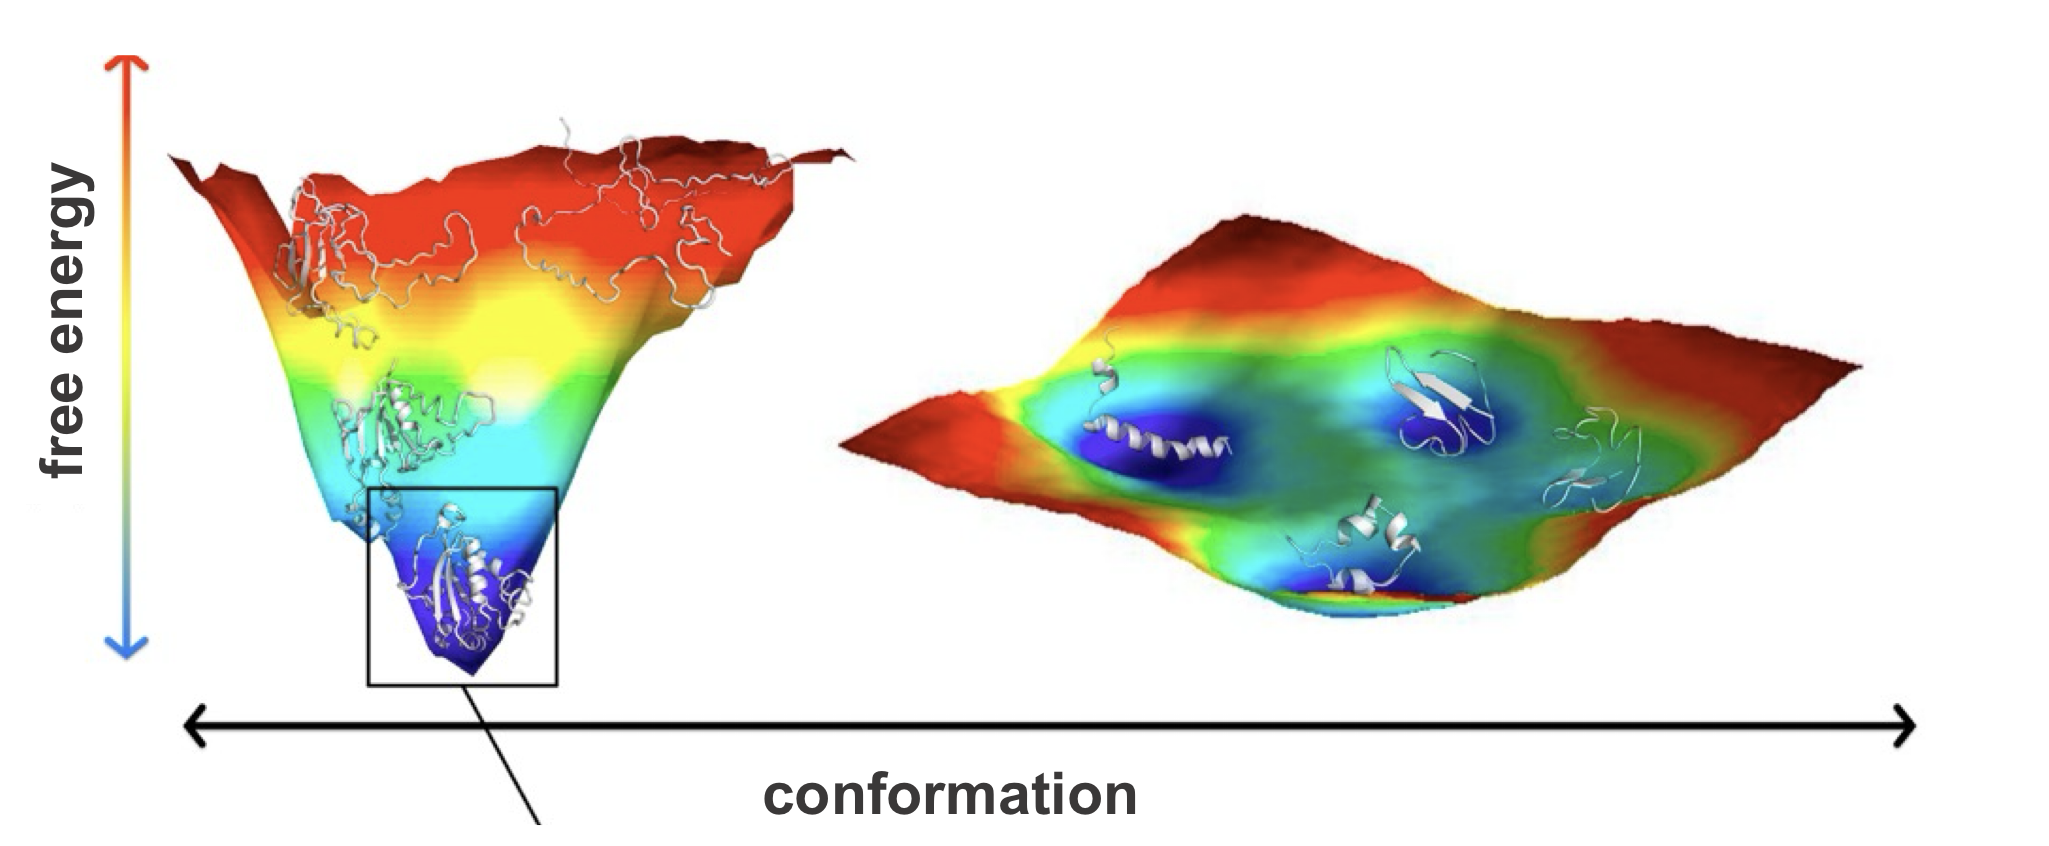
\includegraphics[width =0.8\linewidth]{slides/conformational_ensemble/continuum.png}
    \caption*{}
    \label{fig:placeholder}
\end{figure}
Professor: I will show you immediately another scale that refers to proteins that like to sample this kind of rough surfaces where there is kind of a weak funnelling, okay? And these proteins this was computed like a statistics from all those sequence that were experimentally found to be this kind of floppy thing that we call intrinsically disordered.

Professor: And if you were kind of a familiar with the—familiar with the one-letter codes you can find many correlations, okay, between—sorry I need to define better what is on the Y-axis. So this is not a simple composition but this is a difference between the composition of these disordered protein set minus the globular set normalized.

Professor: So basically when you see a depletion, it means kind of exactly the difference between this surface, I mean protein sequences obeying this surface versus this surface, okay? And this is an extremely simple analysis. So you collect the sequences obeying this, collect the sequences obeying this, you make a—you make the compositions then you compute the differences one by one between the compositions and what you get is this plot.

Professor: So basically these residues here involving the aromatics you recognize phenylalanine, tyrosine and the double ring the tryptophan then the small hydrophobics here they are all depleted which means that they don’t have sufficient amount of—of these hydrophobic residues to form the core. This is what it means and you see in particular the big ones are missing.

Professor: Okay? And in contrast they are enriched in the charged ones K, R the positive ones E and D these are the negatively charged ones and there are some others that you may recognize from the last week like glycine—which is a very flippy floppy residues because it doesn’t really have a sidechain.

Professor: More recent analysis puts glycine here. And then proline, you remember this is the five-membered ring when the residue binds to the main chain and I also told you that this has particular conformations. So it’s interesting. There are some others that are a bit more difficult for you to explain but for example this is serine which can be post-translationally modified you can add a phosphate group and then the conformational properties would be different.

Professor: So I mean this is just like a first baby step I would say, you know, to show you how bioinformatics may work. But I mean of course this is a simple analysis a primary school student can do it. It’s you know computationally nothing. Still if you are doing it good, you may explain some of the very inherent physics of the properties. Again, the goal was to compare proteins that are to be paying funneling.

Professor: Yes. So it means that they don’t want to adopt one structure. They adopt—I mean nothing adopts one structure but maybe some adopt a few and some like hundreds. And these proteins don’t want to have a few they want many. Okay?

Student 4: And this is correlated with the fact that they have more charged amino acids?

Professor: Exactly because the charged amino acids are like water. They don’t want to come together simply they refuse. And they don’t have also the core, they—they miss, I mean not miss but—but they are depleted in hydrophobic residues that would provide this hydrophobic effect.


\paragraph{Functionality regime: change a little, not too much}
Well, as I said, evolution will be a major argument today. So, what you need to understand is as follows. For a protein to function, there is a regime. Of course, when the protein looses too much stability, it looses its functionality. But the problem is that there are some aspects of the function—for example, dynamics, some conformational changes of regulation—that cannot be achieved if the protein is too stable. So, there must be a regime, okay, where the protein is kept for that particular functionality. And at that regime, the protein can accept many mutations which doesn't really change its whole organization but keeps it rather adaptable depending how the conditions are changing.

\paragraph{Difference is enough for specificity? }
I was lucky enough a few years ago working with a pioneer of this theory, and what we tried to explain that, okay, if proteins are frustrated, uh how come that they are specific? If they are not optimal, then how come they are specific? And we computed this kind of—this is a same protein with two different substrates, I think this is a translation initiation factor. And anyway, what you see here on the two triangles, these are contact maps with two different substrates. And what you see also, it's full of red, it’s full of frustration, so it's not optimal at all. But you can even see by eye—but obviously we can compute—that the pattern of the red dots are different. So, it's not optimal, not optimal at all, but it's different. \textbf{And difference can be enough for specificity.} So, we have not finished this study yet; if anyone is interested, it's open.


\paragraph{Surrounding environment can change the shape of the energy landscape}
Student 2: I have a question. Once we have a single protein—so it’s amino acid chain—is the energy landscape fixed or for example some changes in the environment can change it?

Professor: I understand your—you are asking such a difficult question. It’s a very good question, a very, very difficult question. So, what you typically do is that you write your potential as a sum of terms, each accounting for some interaction - and then you add at the end a factor that is coming from the environment. So maybe interaction with a solvent, interaction with an ion, interaction with something. And then things change.


Professor: So you can, you know, you can play and nature plays. That's the very important thing. Nature plays because we must be adaptable. We, including us as an organism, including us as cells, including us as individual proteins within our cell. And this is amazing thing. This is amazing thing and I think because you are physicists and you can truly understand the valid nature of these landscapes, you can appreciate the complexity coming from this little noise — rather I don’t know shouldn’t be noise it’s essential for our life, but this little variations that are without those we would not be alive. And that’s fantastic how to create something which is optimized largely, but just largely but not fully. This is amazing. I mean if you think about it you can spend days thinking about it. It’s a miracle really how to select—because if it’s too much it’s not good. It’s just right. It’s just right. I can speak more later about it or we can chat about it. It’s very interesting.


\subsection{Forces that drive the folding process}
So, first we speak a few words about—about the organization, about thermodynamics, okay, before touching the question of the folding itself. So, obviously we are somehow optimizing, but again not super-optimizing the free energy, okay? So, there are terms that contribute to the enthalpy and there are terms that contribute to the entropy. 


\paragraph{Interactions}
So, one of the key things is hydrogen bonding, okay? This is what keeps proteins kind of stable. Although the overall stability of a protein—let’s say a protein of 300 residues—the overall stability of a protein is around like maybe five hydrogen bonds, the energy of five hydrogen bonds. It's marginal. We say it's marginal.
Hydrogen bonds normally means that there is a—there is a donor, there is an acceptor, and this bond is usually shorter—it’s longer than a usual covalent bond, but but is normally shorter than a usual secondary or non-nonbonding interactions. Normally the distance between the heavy atoms is between 2.5 to 3.5 Angstroms, and this is a very—this is a very interesting bond, we’ll speak more about it. This is something crucial. Uh, you had seen the amino acids, some of them are capable of of forming these.

Then we have covalent bonds, okay? You remember cysteine, and uh upon certain bio—environmental change, at certain electro—let's say redox environment, it can form this covalent bond, okay? And I explained to you that this is good because you can even cut—I mean, the protein is kind of a continuous chain or a set of continuous chains, but if you have these bonds you can even make a scission of some parts of the protein and this will keep it intact.

Then we have kind of also non-bonding interactions, and we can say it's separated here, hydrophobic interactions or Van der Waals interactions. There are interesting forms of how we express this, okay? Uh, with the Lennard-Jones potential, Morse potential, we'll discuss it later, but there are some attraction coming from the hydrophobic groups.

And obviously we do have electrostatic interactions.

\paragraph{Constraints on chain rotations}
And uh when I start rotating them, depending what is at the position of R—so which side chains I have—I can have some some bumps, right? If it's too big and I start turning it, then they bump one another and then you can draw basically very limited area along Phi and Psi where actually these transitions are reasonably smooth. So, this chain geometry put some constraint on the protein. There are some regions where it's kind of allowed and there are some other regions where it's not really allowed.

Then there are some other terms that again we will talk about when we construct our potentials. Things that are like two-body interactions—these are bonds, okay?—then angles, so some parameters of the actual molecularity—these are absolutely like chemical terms, okay, like angles. For example, this is a planar ring, a phenylalanine ring, but obviously if I start let's say whatever a little bit tilting it, it's unfavorable, okay?

Or there can be relations between 1-to-4—these are about we call torsion angles. And it's not—it's a small term but it's a very important term because we have many 1-to-4 interactions and in many cases you you must make sure that the 1-to-4—so these are two atoms that are... Sorry. So, you have two atoms that are covalently bound to one another, 1 and 2, and you have two others, let’s say 3 and 4, that are not covalently bound but obviously their position are largely constrained by the fact that you have two atoms bound. And you can rotate 3 versus 4—so you can start rotating it—but for example if this is a big group, when you rotate to here, there can be, you know, some overlap, some unfavorable repulsion. So, the orientation of 3 and 4 is kind of—I’m not saying it's fixed, but there is a certain kind of energy function associated with it. And this is quite important, this is what called torsion.

Okay. So, this is kind of the geometry of the actual residue, okay? And then you build up on it the geometry of the chain, which is some kind of local parameter.

Okay. So, basically all these, let’s say, three major areas would determine something that people associate with thermodynamic stability of the three-dimensional organization.


But then comes entropy, which most people don't really think about, okay, or think about in a very limited way. So, what contributes to chain stability is obviously the mobility of the whole chain. And here you see a structure colored by so-called B-factor, which shows the thermal vibration of each atom in a crystallographic structure. Very soon, next week, you will learn how to make such kind of pictures and how to interpret such kind of pictures. This is rhodopsin, which is a key protein for light sensing. And you see—not so surprisingly—that the inner helices are kind of more rigid and the surfaces—but not everywhere—they are quite mobile. Uh, sorry, this is a pancreatic lipase. So, anyway, there is some kind of entropy term with this mobilities.

\paragraph{Some proteins are extremely mobile}
In some classes of protein—all proteins move—but in some let's say functional classes, okay, they move extreme. And this is when the conformational energy landscape becomes rather shallow. For example, this is a homeodomain. Homeodomains regulate gene expressions and they are very small, they are super mobile, and they they control absolutely crucial processes by some small bits that you don't even see here because you they couldn't determine the structure; it’s just too mobile. But these tails determine something about DNA specificity, whatever. And if you—if you trigger them, if you, you know, play around with that sequence, uh there is this famous experiment that you can grow a leg from the fly's head, okay? So, you can let's say generate this kind of creatures with very small modifications in the super-super mobile part of the of these types of homeodomains.

\paragraph{The Hydrophobic collapse}

However, the major major entropic driving force for making the three-dimensional organization is something that we kind of touched upon last week. You remember when we discussed why we have the majority of amino acids non-polar? Yeah, right? I asked this question and I got a fairly good answer for that. And I told you that this is the so-called hydrophobic effect, which means that when you have such a hydrophobic chain, water molecules are pretty much constrained, okay, if they need to contact. But whenever you can put these chains together, the water leaks to the bulk and entropy increases.

Now this term is very difficult to capture. We will speak about it because I mean once you not speculate but once you try to estimate, calculate the stability of a protein, this this is very important. However, when people determine a protein structure, this this has already been completed, this process, so all those waters are outside. So, it’s very difficult in fact to trace how much water molecules have left, how tightly they were bound, and what is the entropy gain. Normally the gain from the entropy, even if you take a normal protein, okay, not this kind of extreme disordered protein, is comparable to the interaction energies that you that you get from all these kinds of enthalpy terms. Okay?

\paragraph{Marginal Stability}
the marginal stability. Okay? So, at this moment, before being able to run a simulation, you just need to accept, again, that whenever you sum up all the terms for the protein stability, the ultimate value that you get is around between 5 to 10 kcal/mol. This is about the enthalpy of like five hydrogen bonds.




\subsection{The pathway determines the final folded state}

\begin{figure}[h!]
    \centering
    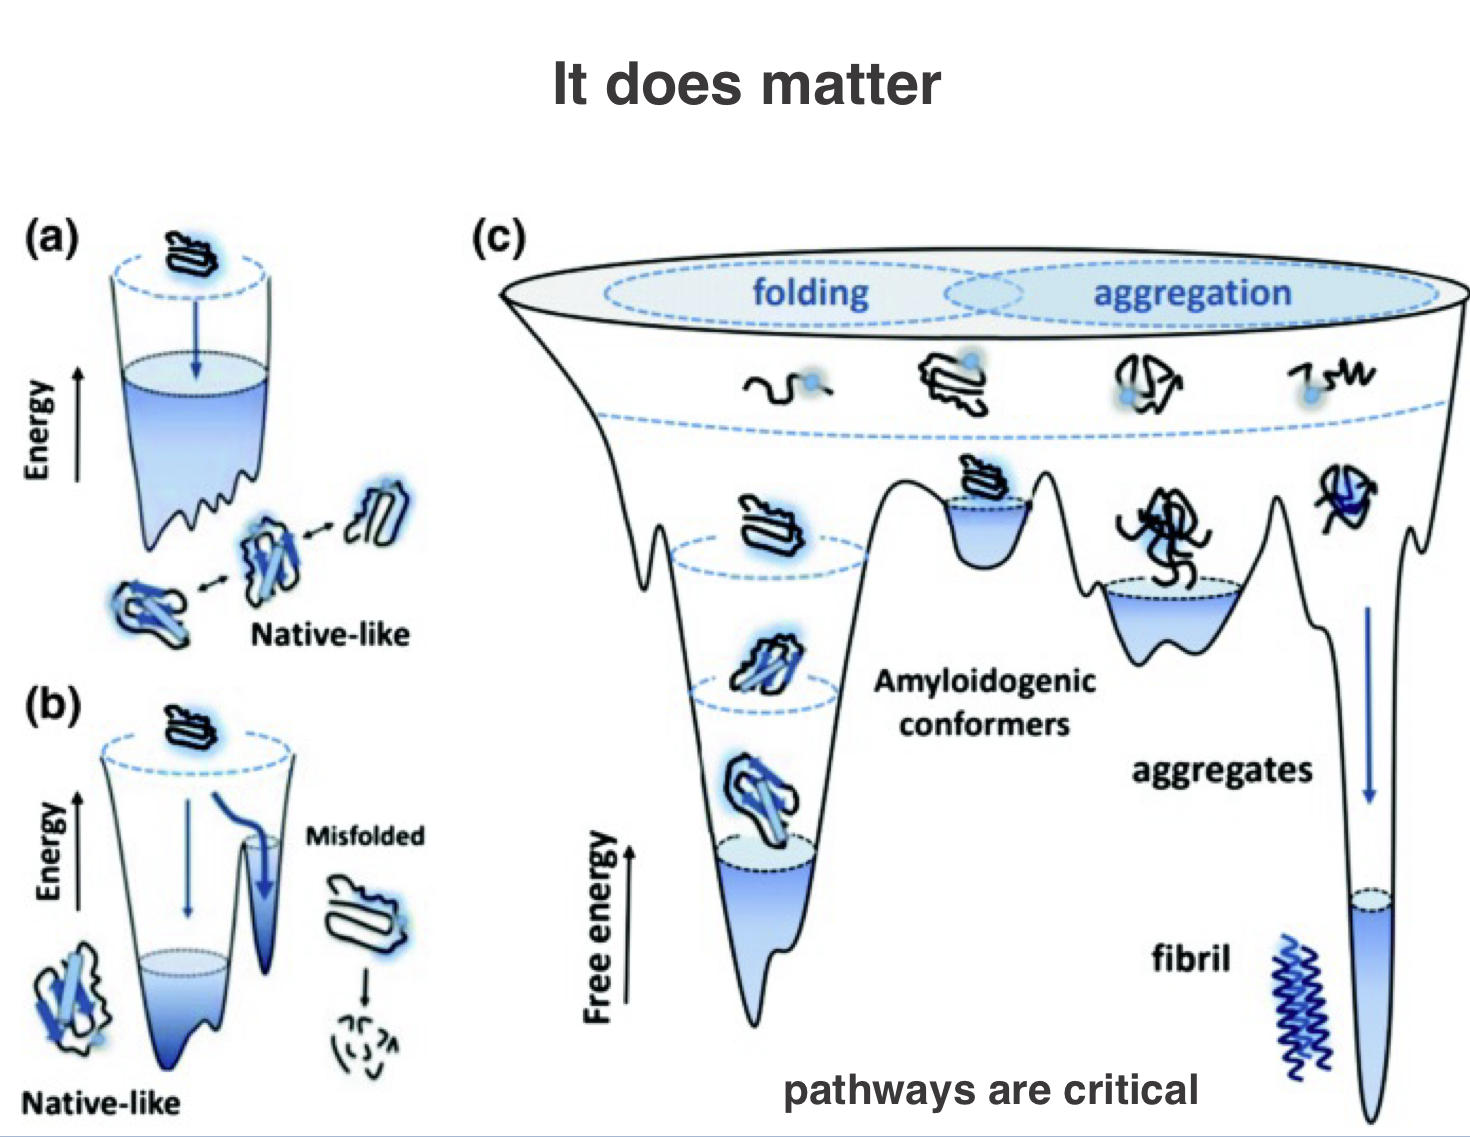
\includegraphics[width=0.5\linewidth]{slides/conformational_ensemble/drawing_different_landascapes.png}
    \caption{}
    \label{fig:placeholder}
\end{figure}
Professor: Okay. So let—let’s go back to the problem. I’m trying now, most argumentation I’ve used until now they were for the thermodynamics and I just told you that some people because of the kinetics used very strange thermodynamic arguments but now I—I full—with full faith I—I would like to address the—the kinetics.

Professor: Okay? So anyway, definitely the point is that it’s in the motion. So when, you know, you construct, you put all these units together, whatever grammar we have—you put and then you need to organize. So definitely—I’m making of course very simple—definitely it’s something that you—that all the bits, all the atoms, all the bonds, all the groups have to move, okay?

Professor: And there are different time scales as you see here. I mean this is again just a very theoretical nanosecond, picosecond and so on. Separated with some barriers but this gives kind of a bit of a let’s say, I don’t know like a scale, okay? Just to imagine. Okay? So you need to move basically from the individual vibrations, for example vibrations of hydrogen bonds, okay? To actual breaking rotations—it’s even—this one even doesn’t include all the—all the relevant motions that you need to consider but maybe giving you some idea. This sidechain fluctuation can mean that you know if you have a big group at the end it’s rotating, whatever. And but you can see already that we are moving from picosecond, we are here nanosecond time scale. Then certain not the whole protein but some domains rotate, okay?

Professor: And then there can be conformational transitions. Here it said microsecond but even can be—can be longer, even can be seconds or even minutes. Okay? So all this when you try to organize that chain that you know we dealt with it like a complex grammar, a complex language, okay? Then let’s say you want to construct a chapter or you want to construct just a section, you need all these motions basically physically to put them together.

Professor: Why and how to put? It’s again that’s a thermodynamics argument but at the end of the day you need all the—you need to consider all these motions. And that’s kind of—the—I’m just jumping. That’s kind of the—the key problem again because that’s already a huge enormous problem of what should contact finally with what, what frustration we should leave and so on.

Professor: But at the end of the day how the protein can reach that state within the time scale that is meaningful for our life, meaning that it around millisecond everything is completed. Okay? But these things cannot occur completely simultaneously. These things cannot—some of those are obligatory, you know, in a—in a consecutive manner. So it’s—it’s a huge problem actually. And without correct folding well we will mention what happens.



\paragraph{The path taken can totally change the output}
Professor: Now the question is, does it matter? Let’s ask that first. Does it matter—I mean I was telling you yes, post-Dill believes in this multiple state but does it matter whether there is one pathway or there are multiple pathways or what do we reach? First let—let’s ask this simple questions. Does it matter? It does matter. 
Professor: And also for the proteins it’s the same thing. The protein for example is very—in particular in the cell is very much attracted to—to make these very tight cross-beta structures. Again I’m calling your attention to this secondary structures file that I posted. You see more if not more pictures about this, okay? This is an extremely tight and stable conformation simply because even you can see by your eyes—it’s a very close contact between the chains so the water molecules basically leave completely. Hydrophobic factor is extremely large. So the—once this is formed this is irreversible. 


Professor: So the protein may try to walk like—my beloved example are mountains. So you know you try to walk from one valley to another valley. There are high peaks. Let’s say you are not an adventurer at this moment you don’t want to go to the peak, you just go through the saddle. Still—still if you go and then each of the class members you won’t go in exactly the same way. You will a little bit explore. Nevertheless if you are without a helmet, without an equipment, you won’t go to the—to the peaks. You will explore more or less the same region. Within that region you move stochastically but it’s unlikely that you end up in any of the peaks.

\paragraph{Folding stages exist but are not so cleasly distinguishable}
So folding qualitatively can occur in many different ways. Initially people thought 'Oh, proteins can form helices, beta strands, they are formed and then they come together' with diffusion and collision. \textbf{However, because of frustration the global organization sometimes overrides whatever is happening at the level of the secondary structures.} So maybe if I cut this protein at this point, I would have this nice helix. However when I fold up everything completely, it’s possible that I’m losing this helix completely because the local contact, the local hydrogen bonds may be less favorable than let’s say the contacts of this one with some turns or whatever. But to some extent the secondary structures are preserved. \textbf{Interestingly, for those proteins that have this very shallow landscape, okay, the secondary structures are better preserved than those proteins that are very nicely packed.} This is something that you can only prove by calculation. 


\paragraph{Experimental stuides of the folding process}
Professor: Well mostly I will try to say something from the point of view of theory, but I also mention because that’s the correct way, I also mention that it’s possible to approach some bits experimentally.

Professor: Simply you need to consider the process. This is a folding process, okay? So from an unfolded state to something which we call a molten globule. Okay? So here it’s completely extended and disordered and this one is still disordered. So the—when we say disordered it means that the—if you define—okay.

Professor: In proteins of course you can define the order by the fixed, let’s say, position by the—by the depth of the valley and by the—by the barrier. But there is another way to define it. And the other way is that in the final protein if you make a catalog of all the interactions that are possible—not are possible but you observe, I don’t know, residues from 1 to—just for simplicity 100, okay?

Professor: And then hydrogen bond between 2 and 24, I don’t know, electrostatic interaction 4 whatever. Basically you can generate some kind of a contact map. That’s—that’s your order. This catalog is your—your order. If you have no fixed catalog but you have 2 interacting not only with 24 but with 53 and 72 and 91 and whatever, then it means it’s disordered.

Professor: This is kind of the—the nomenclature used. Okay? But in this case it’s compact which means that the hydrodynamic radius is—is already small. Okay? So this is about tenth of a microsecond. And then, but this is smooth. With—quasi without barrier. And then from a molten globule to reach a kind of compact ordered state when you fix, okay, you go through an activation energy because some parts you need to expose and other parts you need to kind of repack. And this comes with an activation energy so this is much slower. This is three orders of magnitude slower. This is a millisecond.

Professor: So therefore if it—this is slow you can capture something here and basically what people do experimentally that they make a specific change, a specific mutation in a protein and see how this barrier changes, how the time basically changes, okay, through this transition state.

Professor: And basically they measure the time, okay? And if they make one change this more or less tells the involvement of that region in forming the final—final structure. Okay? And basically if you do a systematic study you can do systematic protein mutations—Herserilant first he invented this methodology it’s called phi value analysis—basically you can tell whether a certain contact was before the transition state or after the transition state because those ones that affect, they were before, those ones that don’t affect, they were after. That’s so simple.

Professor: And this was a very—I mean many people were doing it. Many people it’s like labor. But it turned out that basically this was their favorite enzyme. But it turned out basically that when you start with this very wide region, very few contacts, less than 20percent of the contacts are formed and they already kind of fix the protein towards the final—final state. This is something very interesting.

\subsection{Some facts about hydrophobicity}
Professor: So very small fraction of the contact can be formed before the protein actually reaches its state. I think I don’t need to spend more time. Most of them are related to hydrophobicity, okay? Let’s—let’s skip this now.

Professor: However when we think about the hydrophobic effect and we think about this—this energy that basically the entropy that comes from the released water, we should not exaggerate. We should not exaggerate in a way that there are still water molecules within the protein, okay? The so-called buried waters. And they can be very important because otherwise you would need to pack the protein too tight.

Professor: The protein is normally quite tight in the except of fibrous proteins but you need the waters inside you need the cavities either to mediate the hydrogen bond or basically to fill up that space. Okay?

Professor: There is one simple way that you can also use to estimate the impact from the water that is released and this is the solvent accessible surface or SASA. So basically you can—I mean these are complex geometries but anyway you can estimate what is the surface of the protein that got actually buried without these water molecules that are inside.

Professor: And you consider this is like a water molecule represented by a sphere and you can basically roll this water molecule through all the possible and accessible surfaces, okay? And then it gives you kind of an estimate about the hydrophobic effect in the protein that you investigate in case it’s packed.

Professor: Okay, let’s—let’s keep this is better for the simulation. Now there are—we mentioned this before—there are hydrophobicity scales, okay? And there are many different kinds but basically this is something that you can measure and we will do either next week or the week after some sequence-based predictions, you will see we will use different kinds of scales, but basically these are determined between partition—I mean based on the partition coefficients between some hydrophobic compound and—and water, okay?

Professor: And you can see here, I hope soon you will recognize the one-letter codes that these are highly charged and these are aromatic, these are small hydrophobic and so on. So you can see more or less this scale that can drive the compactness.

\paragraph{The p53 protein is related to half of human cancers}
Professor: Yes. Okay. So for example we talked a little bit about p53 I think before and maybe we will have one simple practical related to it. So this is for example a representative of—of this class and what you see this spaghetti this is not a drawing rather it’s a representation of the ensemble that was detected by different kinds of biophysical techniques and the ultimate ensemble was generated by computer simulation.

Professor: So normally when you have these shallow things, okay, they not only let’s say form conformational ensembles they are ideal for all kinds of regulations because you can very easily shift these ensembles. Of course you can have plasticity in the interactions, okay?

Professor: And unfortunately they approach promiscuity and disease. I mean the binding promiscuity causes disease. For example I—I mentioned to you that the mutations of p53 are involved in about half of the human cancer.

Professor: Okay. I posted a full slide series about this kind of proteins, okay? You can read more about it. If we have time or if you are interested I can give extra lectures it’s not a problem. And you know I can get you more familiar with those.

Professor: But for the moment what you need to understand that this kind of protein dynamics can get a little bit extreme, okay? Pushing or maybe washing away the boundaries of the deterministic relationships putting it more to the stochastic. Okay?

\paragraph{Mathematical modeling of the hydrogen bonding term}

Professor: Now—that was one of the I would say earliest problem of all the simulations to define these surfaces properly so that they properly represent the hydrogen bonding itself. And this is a long story and maybe because I—I see I a little bit run out of time I—I will detail it more when you learn how to construct a force field but—I tell the bottom line of this.

Professor: So initially people thought 'Oh, I need to construct a term for the hydrophobic interaction, I need to construct a term for the electrostatic interaction and plus I need to do something for the hydrogen bonds' and that’s the way how to—basically the—the potential energy surface would—would allow these transitions from coil which is kind of a random thing to—to a relatively well-defined structure.

Professor: And it had been a tremendous—a tremendous let’s say landmark that you don’t need, you don’t need these terms at all. You can basically construct a very simple energy landscape for the hydrogen bonding in base based on the simple Lennard-Jones potentials and electrostatics and—

Professor: Well it was a very—I mean it was the how to say the heroic age of biophysics. So the whole thing started early '70s culminated this Nobel Prize unfortunately the key person has not—has passed away before. But anyway that was a key point to run and to model any kinds of simulations any kinds of speculations to treat the hydrogen bonds not as separate terms but as sums of—of simple electrostatics and—and Van Der Waals maybe this I will just mention to you.